\scanpage{40}
On obtient ainsi
\begingroup\csname tagsleft@true\endcsname
\[
f(t)=\frac{1}{3\sqrt{-3}}\frac{(t+1)(2t-1)(t-2)}{t(t-1)} \tag*{(10)}
\]
\endgroup
et par suite
\[
\boxed{\unsure{\rho^*(t)|p^*(t)}=(gf)^*(t)}\!\boxed{=j=\frac{1}{-27}\left(\frac{(t+1)(2t-1)(t-2)}{t(t-1)}\right)^2} \tag*{(11)}
\]

Cette formule, comme il se doit est définie sur $S$ lui-$=$, et non seulement sur $\unsure{\bar S|J|S|T|S'}$ ! Elle définit un revêtement galoisien de groupe $\mathfrak S_3$ de \deleted{$\unsure{(G_a)_S}$} $P^1_S$, \inserted{à partir de $(G_a)_S$,} qui est non ramifié au dessus de $(G_a)_S-(0)-(1)=(G_m)_S-1$.

\figure{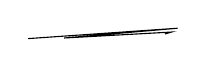
\begin{tikzpicture}[x=1em,y=1ex]\draw[thin] (-3,-.17)--(2.4,.7)--(-1.7,-.12)--(2.18,.38)--(1.94,.22);\end{tikzpicture}}

Comment opère $\sigma$ dans les quotients ?

\noindent\begin{minipage}[t]{.21\linewidth}\vspace{0pt}\scriptsize
\diagram{\begin{tikzcd}[ampersand replacement=\&,row sep=1.3em]
\sigma\quad P^1\arrow[d,"f"]\\
\sigma'\quad P^1\arrow[d,"g"]\\
\sigma''\quad P^1
\end{tikzcd}}
\end{minipage}\hfill\begin{minipage}[t]{.74\linewidth}\vspace{0pt}

On voit que $\sigma'(\infty)=0$, $\sigma'(0)=\infty$, $\sigma'(1)=1$, \deleted{d'où} $=$s formules pour $\sigma''$, d'où \deleted{$\sigma'(t)=1/t$}

\deleted{et d'autre part}
\begingroup\csname tagsleft@true\endcsname
\[
\sigma'(t)=\sigma''(t)=1/t \tag*{(11)}
\]
\endgroup
et il serait facile de passer au quotient par $\sigma$ \deleted{\unsure{de}} en dernier lieu (p.ex.).
\end{minipage}
\figure{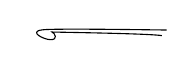
\begin{tikzpicture}[x=1em,y=1ex]\draw[thin] (2.35,.35) .. controls (1.85,.36) and (-1.8,.5) .. (-2.15,.36) .. controls (-2.65,.21) and (-2.08,-.46) .. (-1.85,-.46) .. controls (-1.55,-.48) and (-1.69,.1) .. (-1.79,.18) .. controls (-.18,.11) and (1.78,.02) .. (2.18,-.12);\end{tikzpicture}}
% archive sheet number: 39
